\documentclass[11pt,a4paper]{jsarticle}

\usepackage[dvipdfmx]{graphicx}
\usepackage{graphicx}
\usepackage[top=20truemm,bottom=20truemm,left=25truemm,right=25truemm]{geometry}
\usepackage{comment}

%https://qiita.com/Toru3/items/7ea1342da1e31f0c28c3
\usepackage{fancyhdr}
\usepackage{lastpage}
\fancypagestyle{mypagestyle}{%
\lhead{\thepage/\pageref{LastPage}}%ヘッダ左
\rhead{留学先での研究テーマ 平松信義}%ヘッダ右
\cfoot{}%\thepage/\pageref{LastPage}}%フッタ中央に"今のページ数/総ページ数"を設定
\renewcommand{\headrulewidth}{0.0pt}%ヘッダの線を消す
}
\pagestyle{mypagestyle}

\title{留学先での研究テーマ\\準粒子からなるボース・アインシュタイン凝縮体の光制御}
\author{東京大学工学部物理工学科 平松信義}
\date{\today}
\begin{document}
\maketitle
\thispagestyle{mypagestyle}

\section{光技術を用いたボース・アインシュタイン凝縮の観測}
ボース・アインシュタイン凝縮(BEC)は、低温で近接するボース粒子同士が量子力学的な干渉をして、最低エネルギー状態に落ち込む現象である。ボース凝縮体において粒子はお互いに協調してふるまい、巨視的な量子効果があらわになる。
ボース粒子がお互いに干渉してBECが観測できるための条件は、ボース粒子の波束の広がりがボース粒子間の平均的な距離に対して長いことである。ボース粒子の波束の広がりは、以下の熱的ド・ブロイ長$\lambda_{\rm TdB}$で特徴づけられる。
\begin{eqnarray}
\lambda_{\rm TdB} &=& \frac{h}{\sqrt{2\pi m^* k_B T}}.
\label{eq:lambda}
\end{eqnarray}
ただし$h$はプランク定数、$k_B$はボルツマン定数、$m^*$はボース粒子の有効質量である。温度を低くすれば熱的ド・ブロイ長$\lambda_{\rm TdB}$は大きくなり、ある温度以下でBECの観測が可能になる。また実現できる温度に下限が存在しても、十分にボース粒子の有効質量が小さくまた十分に粒子が密に存在していれば、その系でBECの観測は可能になる。

アインシュタインの1925年の予言以来、BECは明らかな形で確認されていなかったが、1995年に低温の希薄ガス中で観測された\cite{Davis,Anderson}。磁気光学トラップ(MOT)と呼ばれるレーザー光を用いた粒子閉じ込め方法と、蒸発冷却と呼ばれる冷却手法のブレークスルーが、BECの実現につながった。それ以来MOTと蒸発冷却は希薄ガスのBECを実現する標準的な方法となった。MOTは非一様磁場中に偏光した光を入射する手法で、粒子は空間的に束縛されボース粒子の密度は大きくなる。そのあと様々な物質の系でBECは実現されているが、光技術を用いた冷却はその多くで用いられ\cite{ketterle}、BECを実現するために極めて有用である。

またBECに関して現在知られているほぼ全てのことは光を用いた探査法によって得られたたものである\cite{ketterle}。光学測定には接触方式と異なり、系への熱の流入を防げるという大きな利点がある。またボース粒子の時間依存する分布を非破壊に見たり、吸収・散乱からエネルギースペクトルなどを測定できるといった測定の多様さも有利である。実際、希薄ガスのBECの検出には光学系が広く用いられており、後述する励起子のBEC観測実験\cite{Yoshioka}でも励起子の励起と計測に光技術が用いられている。

\section{励起子のBEC}
%励起子は結晶をバンド理論で記述した時に現れる電子と正孔がクーロン引力により束縛状態を作ったものであり、
励起子は準粒子と呼ばれるエネルギー量子の一つであり、結晶中に現れるボース粒子である。
励起子のBECはこれまで理論的に予測されていたが\cite{Blatt}、励起子同士の相互作用から有限の寿命を持っており、ボース・アインシュタイン凝縮体が実際に形成されるかどうかは自明でなかった。

励起子のBECを検出するために近年まで酸化銅${\rm Cu_2O}$を中心に着実な実験研究が進められてきた\cite{David}。しかし励起子は相互作用するため、多くの物質でBECを実現するには温度1K 以下の超低温が必要で、実証的な実験は困難だった。しかし近年BECに伴う緩和爆発が検出され\cite{Yoshioka}、励起子のBECが発現した実験証拠と考えられている。

これらの一連の研究は低温物理学と物性物理学の新しい可能性を示している。
第一に励起子の多体系でBECを観測できたことは、今後結晶中の他の準粒子に関してBECが実現できる可能性を示唆する。また半導体の非常に多彩な性質は励起子により特徴づけられており、BECを起こした励起子を活用することで新たな半導体デバイスへの応用の可能性も考えられる。
第二に、この実験で重要な役割を果たした励起子の質量は小さく、式\ref{eq:lambda}から熱的ド・ブロイ長$\lambda_{\rm TdB}$は大きい。今後さらなる高温でBECが実現でき、より多様な実験が行える可能性が考えられる。

\section{準粒子からなるボース・アインシュタイン凝縮体の光制御}



\section{筆者のこれまでの経験と留学先での研究}
筆者はこれまで光技術を用いた準粒子の特性評価に関わってきた。
筆者は表面プラズモンポラリトンの特性を体系的に評価し\footnote{研究論文の要旨1 (出版論文の要旨)}、論文に出版した\cite{Hiramatsu}。表面プラズモンポラリトンは金属表面に現れる準粒子である。
アメリカのライス大学で行なった研究では、InSeに現れる励起子の偏光分解分光を行なった\footnote{ 図\ref{fig:poster}: Rice大学で研究発表した際に用いたポスター(参考)}。

また東京大学の卒業研究ではIrTe$_2$の光誘起とに関する研究に関わってきた\footnote{研究論文の要旨2 (卒業研究中間報告書の要旨)}ここで超伝導状態は電子対がBECを起こすとして定性的に理解できる。さらに半導体の光計測技術に関してオーストリアの企業で開発研究に関わり、ヨーロッパ特許を出版した\cite{Etschmaier}。

以上の経験から、本資料に記述したテーマに関して、留学先で比較的スムーズに研究を進めていけると筆者は自負している。

\begin{figure}[p]
  \begin{center}
   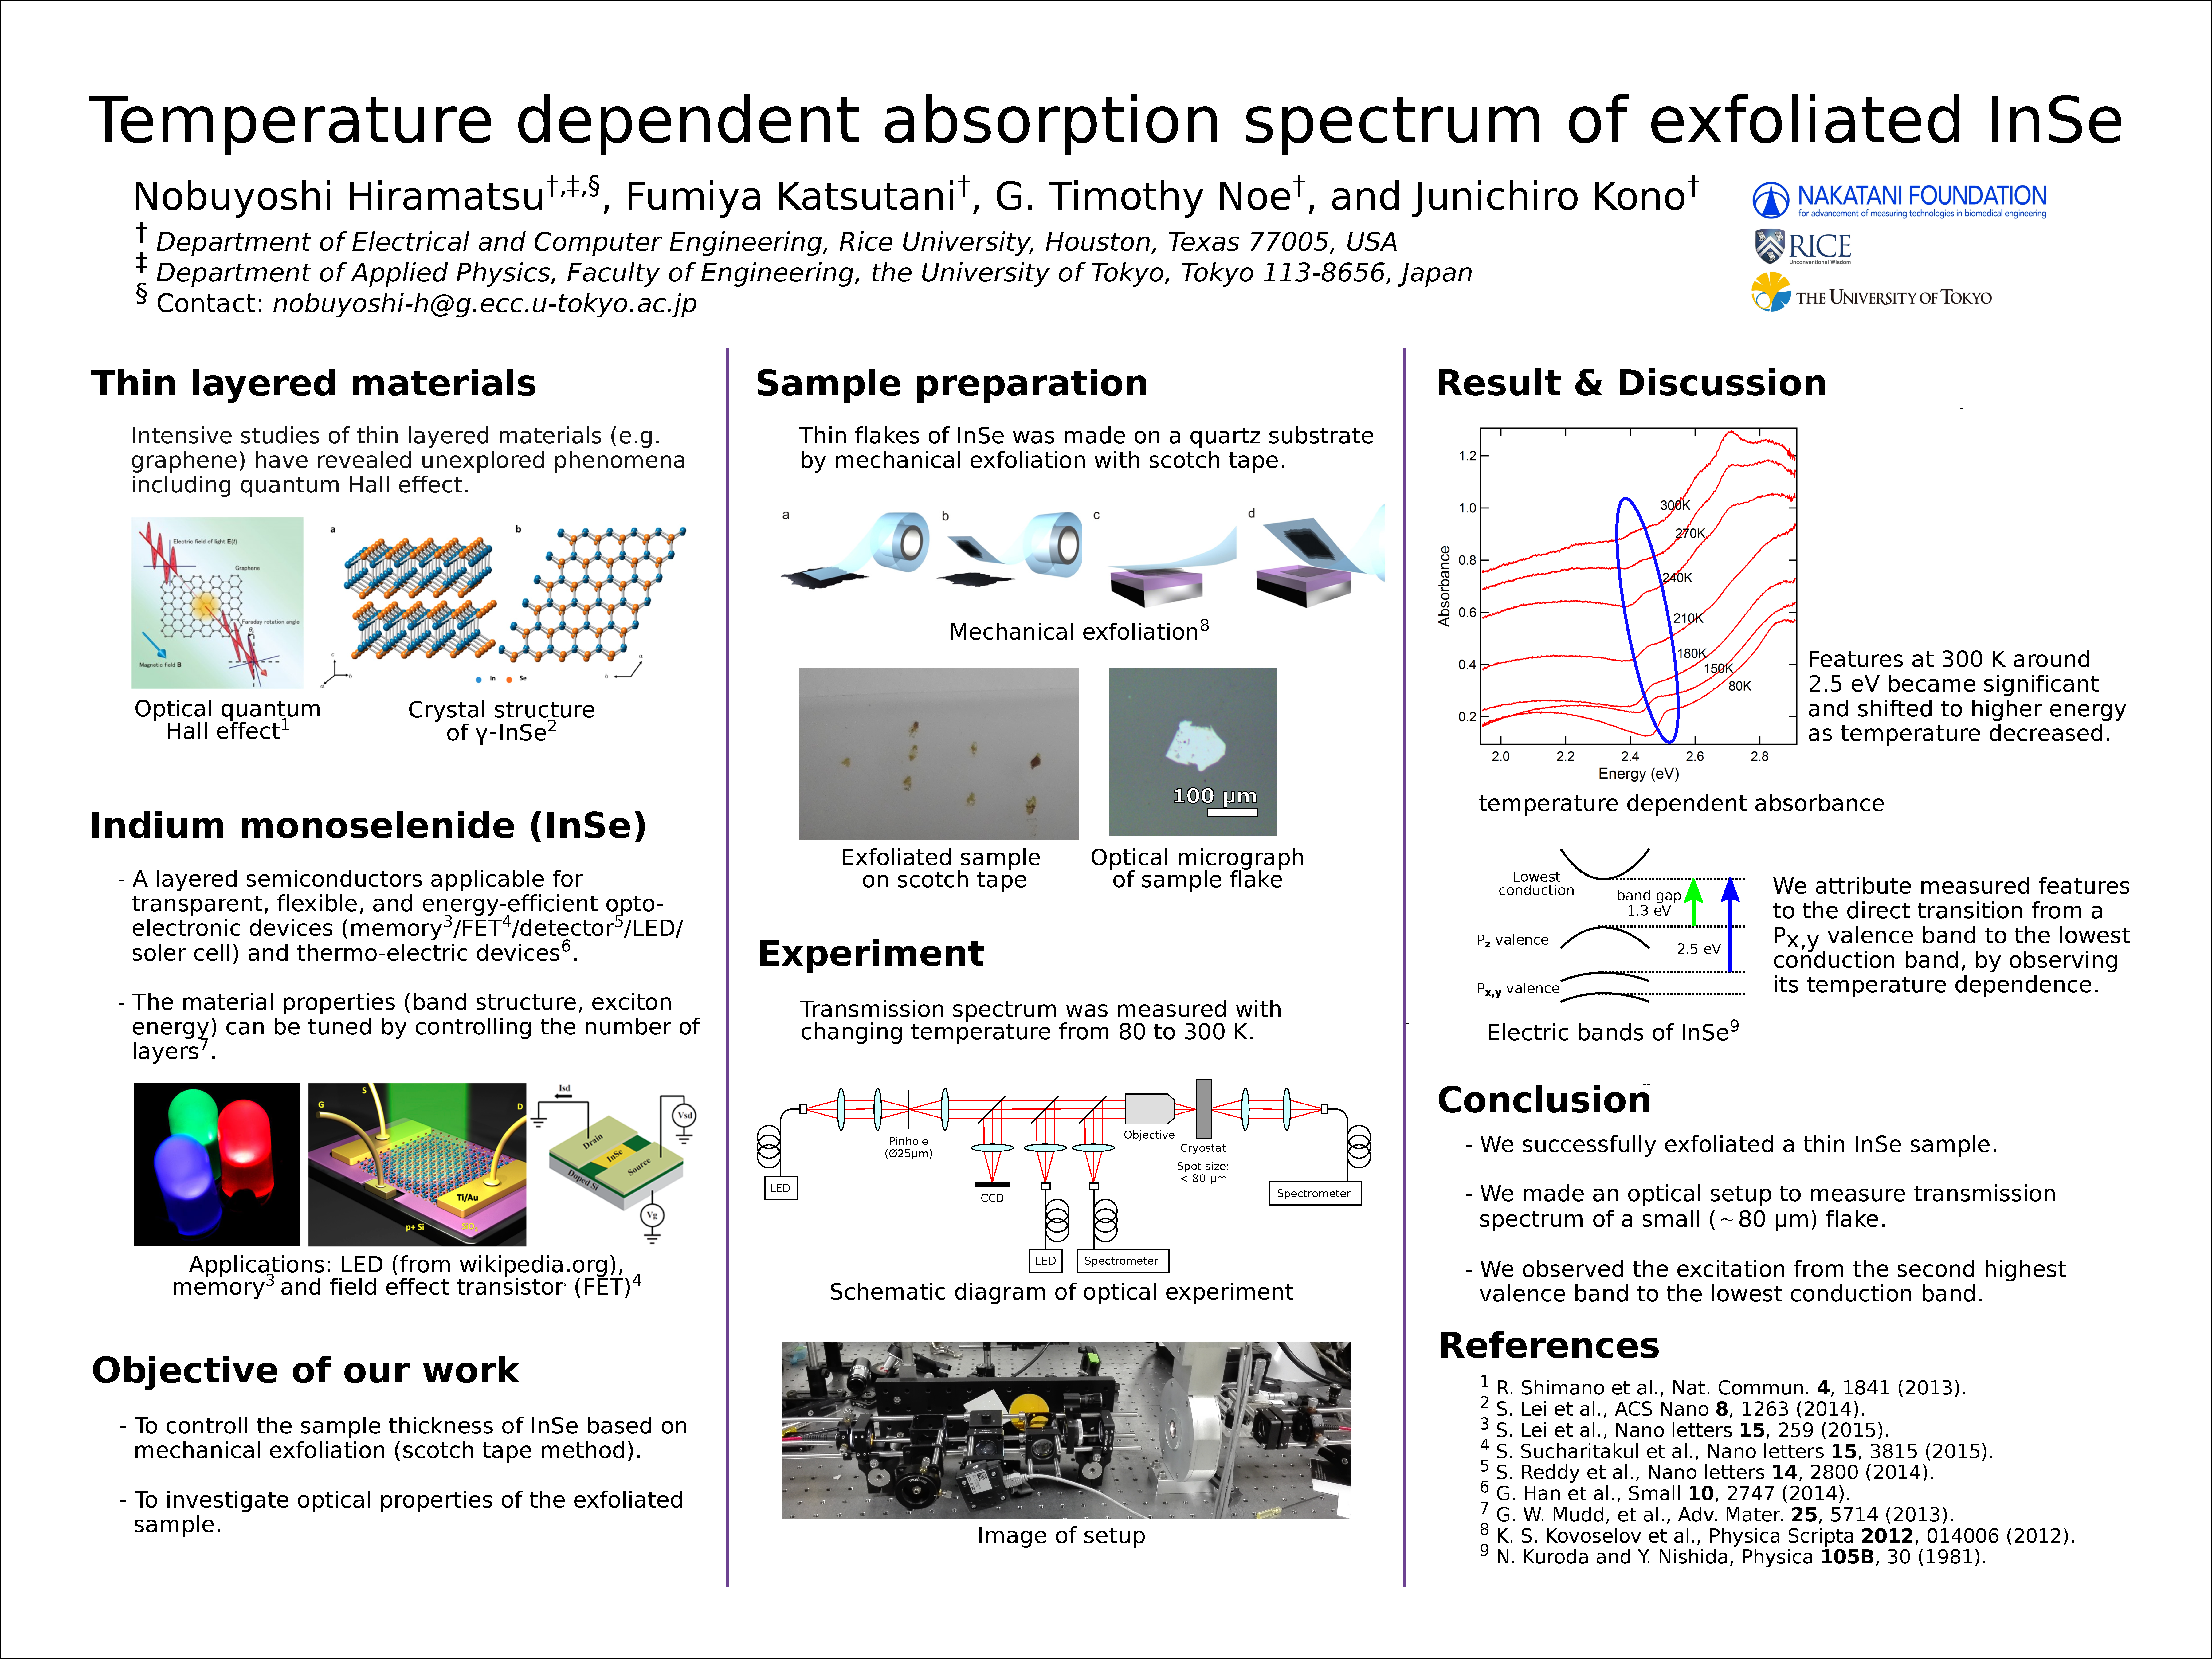
\includegraphics[width=1.4\hsize, angle=90]{poster_submitted.pdf}
  \end{center}
  \caption{Rice大学で研究発表した際に用いたポスター(参考)}
  \label{fig:poster}
\end{figure}




%\nocite{*}
\bibliography{SOP.bib}
\bibliographystyle{junsrt}



\end{document}
%コンパイルの仕方
%1. texファイルを一回コンパイル
%2. bibファイルを一回コンパイル
%3. texファイルを三回コンパイル